\chapter{RESULTS}\label{chapter:results}

In this thesis, we are not looking to obtain the best possible combination of hyperparameters for training loss or model accuracy.
Instead, we want to observe the effects on training with Hivemind when tuning common hyperparameters such as batch size and learning rate and Hivemind hyperparameters such as the TBS.
In this thesis, we analyze the performance and limits of training using Hivemind rather than looking for the best model.

\section{Baseline runs}

We begin this chapter by showing the results that we have obtained with the baseline runs.
As mentioned previously in \autoref{chapter:setup}, all baseline experiments are executed on machines with the same configuration, and the total number of samples processed is always the same.
\autoref{fig:baseline-runtimes} shows the average runtimes for baseline runs in minutes.
As we might have expected, most runs take more or less the same amount of time, as the total number of samples processed is the same for every run
\footnote{
    BS=128 takes more time due to resource contention happening during the execution of the baseline runs.
}.

\begin{figure}[ht]
    \centering
    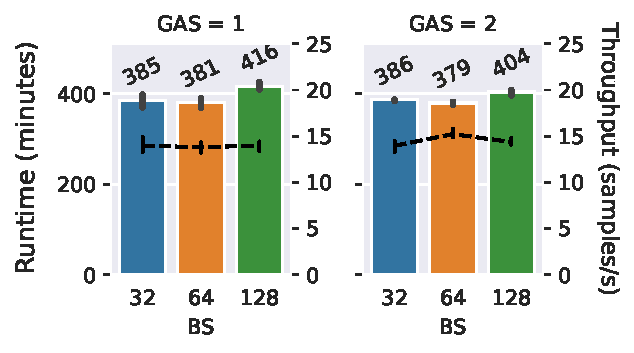
\includegraphics[width=0.6\textwidth]{./figures/06_barplot-runtime_baseline-16vCPUs-GAS-1.pdf}
    \caption{
        Average runtimes (bars) of baseline experiments in minutes.
        Runs are aggregated across LR, with the standard deviation amongst reruns as the black bars.
        The black dashed line indicates the throughput in samples per second.
    }
    \label{fig:baseline-runtimes}
\end{figure}

\begin{figure}[ht]
    \centering
    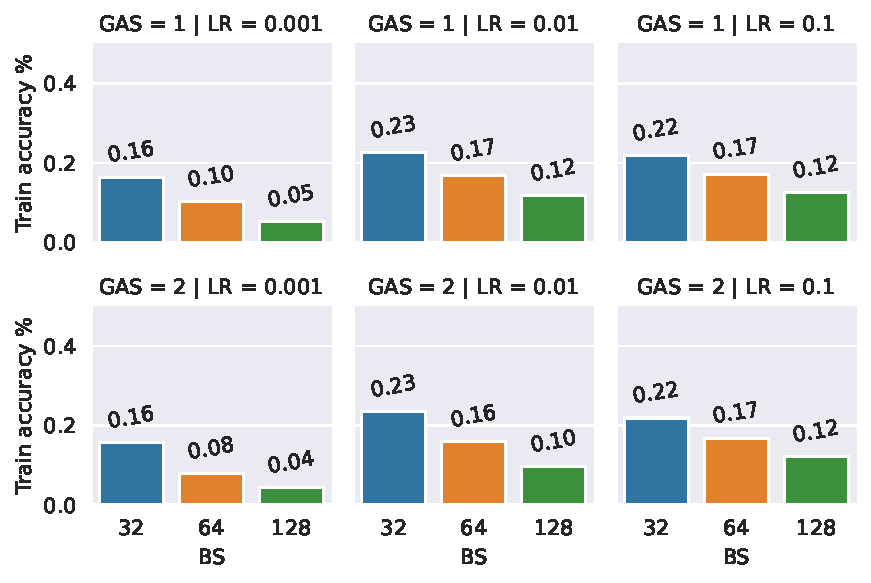
\includegraphics[width=0.6\textwidth]{./figures/06_barplot-losses_baseline-16vCPUs-GAS-1.pdf}
    \caption{Maximum accuracy achieved by baseline runs, averaged across re-runs.}
    \label{fig:baseline-losses}
\end{figure}

Baseline runs do not use distributed algorithms and all Hivemind features are switched off.
However, \autoref{fig:net-recv_baseline} shows that there is some network activity.
On average, every machine receives a constant 1.5 MB/s of data on its network.
This may be due to several factors, such as KVM management data, OpenNebula pings, and CEPH data being read.

In the Setup section, we also introduced our monitoring tool of choice \textit{wandb}.
Because this is an online monitoring tool, some data about our runs is periodically sent to the Weights and Biases server for storage and visualizations.

In \autoref{fig:net-sent_baseline}, which shows the bandwidth used for send operations across all baseline runs, we can observe the bandwidth in MB/s used for each run.
On average, this is roughly 0.02 MB/s on every run, a value that can be mostly attributed to \textit{wandb} and other background monitoring operations such as OpenNebula.

In future sections, we will always account for these effects when performing comparisons with baseline runs.

\begin{figure}[ht]
    \centering
    \begin{subfigure}[t]{0.475 \textwidth}
        \centering
        \caption{Network bandwidth sent in MB/s for baseline runs. Values above 0.07 are hidden. Runs are aggregated across LR.}
        \label{fig:net-sent_baseline}
        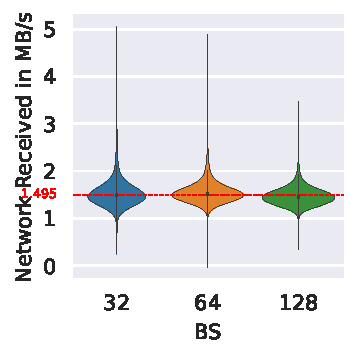
\includegraphics[width=0.5\textwidth]{./figures/06_net-recv_baseline-16vCPUs-GAS-1.pdf}
    \end{subfigure}
    \centering
    \begin{subfigure}[t]{0.475 \textwidth}
        \centering
        \caption{Network bandwidth received in MB/s for baseline runs. Values above 5 are hidden. Runs are aggregated across LR.}
        \label{fig:net-recv_baseline}
        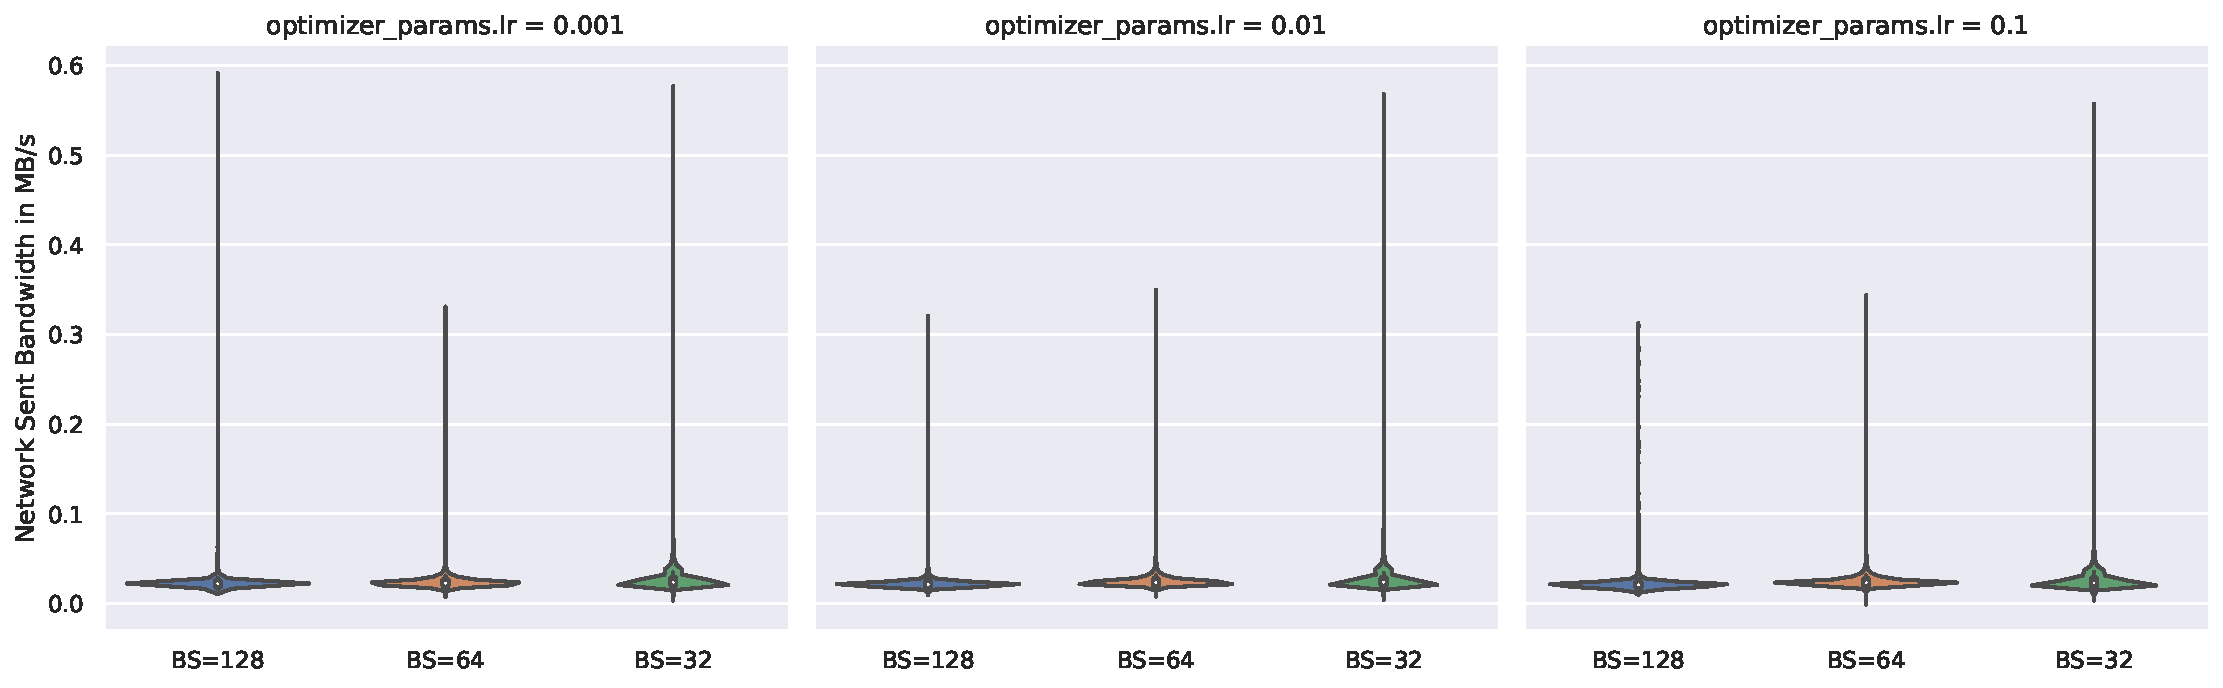
\includegraphics[width=0.5\textwidth]{./figures/06_net-sent_baseline-16vCPUs-GAS-1.pdf}
    \end{subfigure}%
    \hfill
    \caption{Network bandwidth sent and received in MB/s for baseline runs. Runs are aggregated across LR.}
\end{figure}

\autoref{fig:baseline-times-stacked} shows the average times for data load, forward pass, backward pass and optimization step across batch sizes in baseline runs for both GAS=1 and GAS=2.
As we might expect, the time it takes for a single step to complete is linearly dependent on the batch size.
The learning rate (LR) does not affect the time it takes for each step to complete, so we aggregated the runs for each batch size.
By contrast, the number of gradient accumulation steps (GAS) seems to shave off some time for every batch size.
However, the total runtimes in \autoref{fig:baseline-runtimes} do not seem to reflect this improvement.
Because of this, throughout this chapter, we will keep showing GAS runs separately, as it still might affect some other aspects of training.

We further note that each step's average time remains relatively unchanged throughout every experiment, given the same computational power, except for the data load and optimizer steps
\footnote{We will not show anymore the times of every step besides the optimizer step, as they remain generally constant.}.
The irregularity of the storage medium that we used for the experiment, CEPH, is to blame for the slight irregularities in the data load step.
Regarding the optimizer step, its irregularities are due to two main factors: Hivemind settings and overcommitted nodes.

We will explore later in this chapter the effects of Hivemind settings on the optimizer step.
Overcommitted nodes are a consequence of the cloud environment where the machines that perform our experiments are set up.
Because we have limited resources in our cluster, sometimes other researchers may need to overcommit the same node vCPUs to perform their experiments.
This causes several issues when training in a distributed setting with Hivemind, such as nodes not responding for long periods of time, sometimes even minutes.
In such cases, two things can happen:

\begin{itemize}
    \item if the non-responding node or nodes were not participating in an averaging round, other participating nodes will wait for 10 seconds, and then start an averaging round without other nodes;
    \item if the node was actively participating in an averaging round, nodes will wait for the node to come back for 300 seconds or five minutes.
\end{itemize}

Future efforts to replicate the results presented in this thesis may wish to pin their resources to prevent or reduce these issues from happening.

In \autoref{fig:baseline-times-stacked} we can also notice the big impact that data loading has on every step.
Almost 1/2 of the total time for each step consists in waiting for the data to load.
As we increase the number of cores per peer, CPU utilization decreases, as the CPU is idle during I/O wait times and normal operations such as forward and backward pass take less time.
This is a bottleneck that can easily be tackled through several means, such as having a faster storage backend or if that is not available, faster data loader frameworks and algorithms \cite{isenko2022bottleneck, leclerc2022ffcv}.
Future work may make use of local, faster storage backed by SSD to achieve faster data load speeds, helping us rule out the effects of data loading on training with Hivemind.

\begin{minipage}{\linewidth}
    \begin{minipage}{0.45\linewidth}
        \begin{figure}[H]
            \centering
            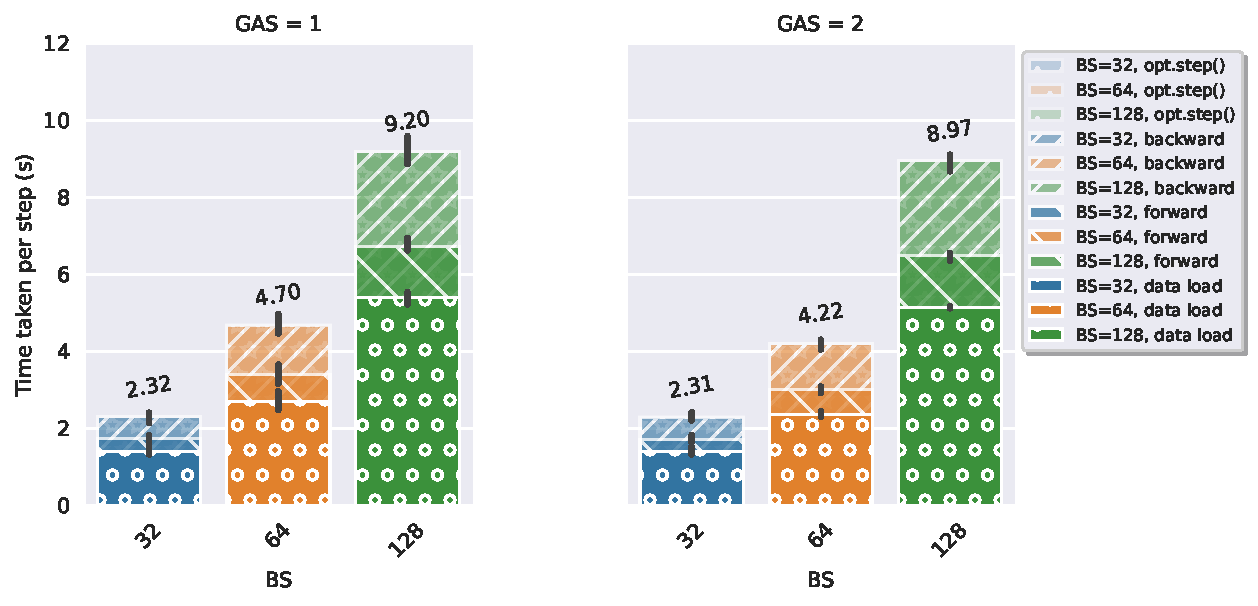
\includegraphics[width=\textwidth]{./figures/06_barplot-times_baseline-16vCPUs-GAS-1.pdf}
            \caption{
                Average times of step data load (red), forward pass (green), backward pass (orange) and optimization step (blue) baseline experiments in seconds.
                Runs are further aggregated across LR and the standard error amongst runs is shown with black bars.
            }
            \label{fig:baseline-times-stacked}
        \end{figure}
    \end{minipage}
    \hspace{0.05\linewidth}
    \begin{minipage}{0.45\linewidth}
        \begin{figure}[H]
            \centering
            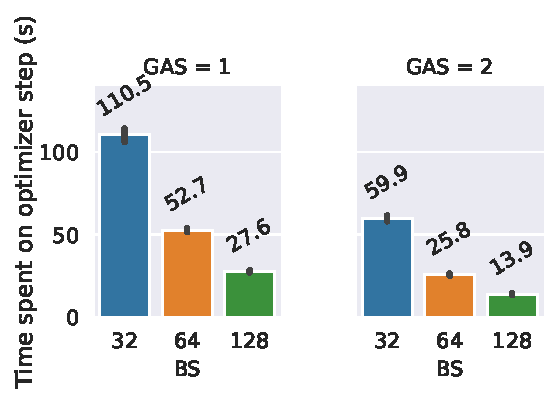
\includegraphics[width=\textwidth]{./figures/06_barplot-times-opt_baseline-16vCPUs-GAS-1.pdf}
            \caption{
                Cumulative time taken by the \texttt{opt.step()} for every batch size, in seconds.
                Runs are further aggregated across LR and the standard error amongst runs is shown with black bars.
            }
            \label{fig:baseline-times-opt}
        \end{figure}
    \end{minipage}
\end{minipage}

Finally, we zoom in on the effect of GAS for baseline runs on the optimizer step times in \autoref{fig:baseline-times-opt}.
The graph shows the total amount of time spent for each run to perform \texttt{opt.step()}, grouped by LR.
As we might expect from \autoref{alg:grad-acc-training}, doubling GAS led to half the time spent on the optimizer step, as it is called exactly half of the time.
Furthermore, as we increase the batch size, we also reduce the amount of time spent performing the optimization step.
Because backpropagation scales with the number of outputs, performing the optimization step does not scale up with the increased input size.
In the next sections, we will further analyze the effects of using GAS together with other Hivemind settings.

\section{Focus on effects of batch size, learning rate and target Batch Size}\label{sec:focus-effect-bs-lr-tbs}

Batch size and learning rate are some of the most fundamental hyperparameters to tune when training a neural network to obtain good training results.
Tuning the learning rate should not impact training performance directly, but it can help to better understand how to tune it for different settings combinations while using Hivemind.
As specified previously in \autoref{chapter:setup}, the reference optimizer algorithm is the stochastic gradient descent (SGD), which is wrapped around the \texttt{hivemind.Optimizer} class.

The batch size determines how many samples are being processed in a training loop.
In Hivemind, this has the consequence of reaching the TBS in fewer steps, but not necessarily in less time.

\begin{figure}[ht]
    \centering
    \foreach \gas in {1, 2}
        {
            \begin{subfigure}[t]{0.4 \textwidth}
                \caption{}
                \includegraphics[width=\textwidth]{./figures/06_barplot-runtime_gas-\gas_2-peers-8vCPUs.pdf}
            \end{subfigure}
        }
    \caption{Runtime decrease in percent for Hivemind runs with 2 peers and 8vCPUs relative to the baseline runs. Higher is better. Runs are aggregated across LR and the standard error amongst runs is shown with black bars.}
    \label{fig:runtime-decrease_2-peers-8vCPUs}
\end{figure}

\autoref{fig:runtime-decrease_2-peers-8vCPUs} shows the runtimes for Hivemind experiments with 2 peers and 8vCPUs per peer compared to the baseline runs.
Every run shows a substantial decrease in runtime, with $BS=32$ having an average decrease of circa 20\%, $BS=64$ of circa 30\% and close to 40\% for $BS=128$.
But can we just expect such a high increase in performance for free when turning on Hivemind?
There are two important factors to take into consideration before making a such claim.

\begin{figure}[ht]
    \centering
    \foreach \lu in {True, False}
        {
            \begin{subfigure}[b]{0.475\textwidth}
                \centering
                \caption{}
                \includegraphics[width=\textwidth]{./figures/06_barplot-loss_gas-1_lu-\lu_2-peers-8vCPUs.pdf}
            \end{subfigure}
            \hfill
        }
    \caption{GAS=1, accuracy decrease in percent for Hivemind runs with 2 peers and 8vCPUs relative to the baseline runs. Higher is worse.}
    \label{fig:loss-increase_gas-1_2-peers-8vCPUs}
\end{figure}

\begin{enumerate}
    \item Data loading in the baseline runs takes 1/3 of the total time per step as shown in \autoref{fig:baseline-times-stacked}.
          Parallelizing data loading indeed speeds up the overall runtime for each run.
          With further experimentation that is outside the scope of this thesis, it might be possible to reduce the data loading step with local parallelization techniques and faster storage.
          Reducing the data loading step might help rule out the possibility that we only see runtime improvements because of the effects of loading more data in parallel.
    \item The results in \autoref{fig:loss-increase_gas-1_2-peers-8vCPUs} and \autoref{fig:loss-increase_gas-2_2-peers-8vCPUs} shows the hidden impact on accuracy of using Hivemind.
          Nearly all experiments are not able to reach the maximum accuracy set by the respective baseline runs.
          Some experiments \cite{you2017scaling} have shown that large batch training can lead to divergence, and it is possible to reach the same model accuracy just by training longer.
          Others \cite{DBLP:journals/corr/KeskarMNST16} argue that longer training with larger batch sizes might lead to overall worse generalization capabilities for the model.
          Proving the effects on accuracy and model generalization is beyond the scope of this thesis.
\end{enumerate}

\begin{figure}[htb]
    \centering
    \foreach \lu in {True, False}
        {
            \begin{subfigure}[b]{0.475\textwidth}
                \centering
                \caption{}
                \includegraphics[width=\textwidth]{./figures/06_barplot-loss_gas-2_lu-\lu_2-peers-8vCPUs.pdf}
            \end{subfigure}%
            \hfill
        }
    \caption{GAS=2, accuracy decrease in percent for Hivemind runs with 2 peers and 8vCPUs relative to the baseline runs. Higher is worse.}
    \label{fig:loss-increase_gas-2_2-peers-8vCPUs}
\end{figure}

Depending on the optimizer used for training a neural network model, the number of parameters can become huge.
When performing an optimizer state averaging state, sending a high amount of parameters can lead to high communication overhead, and thus, reduced performance \cite{10.48550/arxiv.1705.08741, DBLP:journals/corr/abs-2003-11316, 10.5555/2999134.2999271, DBLP:journals/corr/abs-1811-03600}.
However, this effect is almost non-existent for small neural networks such as ResNet18 \cite{DBLP:journals/corr/abs-2006-10103}.

\autoref{fig:net-recv-sys-bandwidth-mbs_2-peers-8vCPUs} and \autoref{fig:net-sent-sys-bandwidth-mbs_2-peers-8vCPUs} show that the bandwidth utilization is very low for a local network such as that of the setup of our experiment.
Consequently, none of our Hivemind experiments ever reached network bandwidth saturation for both receive and send operations.
Furthermore, the Hivemind settings of our experiments do not allow overlapping training operations with averaging operations, which are all executed during the \texttt{opt.step()} call.
Gradients are thus sent and received in a single step rather than in the background, which in our experiments did not lead to any discernible bottleneck.

\begin{figure}[ht]
    \centering
    \foreach \gas in {1, 2}
        {
            \begin{subfigure}[t]{0.4\linewidth}
                \centering
                \caption{}
                \includegraphics[width=\textwidth]{./figures/06_net-recv-sys-bandwidth-mbs_gas-\gas_2-peers-8vCPUs.pdf}
            \end{subfigure}
        }
    \caption{Network received for Hivemind runs with 2 peers and 8vCPUs. Values $\geq 10$ MB/s are hidden and runs are aggregated across LR.}
    \label{fig:net-recv-sys-bandwidth-mbs_2-peers-8vCPUs}
\end{figure}

\begin{figure}[ht]
    \centering
    \foreach \gas in {1, 2}
        {
            \begin{subfigure}[t]{0.4\linewidth}
                \centering
                \caption{}
                \includegraphics[width=\textwidth]{./figures/06_net-sent-sys-bandwidth-mbs_gas-\gas_2-peers-8vCPUs.pdf}
            \end{subfigure}
        }
    \caption{Network sent for Hivemind runs with 2 peers and 8vCPUs. Values $\geq 10$ MB/s are hidden and runs are aggregated across LR.}
    \label{fig:net-sent-sys-bandwidth-mbs_2-peers-8vCPUs}
\end{figure}

Taking a look back at \autoref{fig:use-local-updates_false} and \autoref{fig:use-local-updates_true}, we expect that as we increase TBS, we should see the time spent on \texttt{opt.step()} increase.
This is because nodes perform more steps overall, and thus spend more time looking for peers to perform averaging with.
Furthermore, we should see that as we increase the batch size, we also spend less time performing the optimization step, as we do fewer calls to \texttt{opt.step()} in total.
\autoref{fig:times-stacked_2-peers-8vCPUs} shows the cumulative time taken for the optimization step in every run, aggregated per LR.
Generally, we see that our expectations are confirmed across all runs, with some exceptions
\footnote{
    The imperfect environment that our experiments are performed on allows node overcommitting, causing some runs to show increased waiting times.
}.

\begin{figure}[ht]
    \centering
    \foreach \gas in {1, 2}
        {
            \begin{subfigure}[t]{0.35\textwidth}
                \centering
                \caption{}
                \includegraphics[width=\textwidth]{./figures/06_barplot-times_gas-\gas_2-peers-8vCPUs.pdf}
            \end{subfigure}
        }
    \caption{
        Cumulative time taken by the \texttt{opt.step()} for Hivemind experiments with 2 peers and 8vCPUs in minutes.
        Runs are further aggregated across LR and the standard error amongst runs is shown with black bars (continues).
    }
    \label{fig:times-stacked_2-peers-8vCPUs}
\end{figure}

Considerations of training with Hivemind for the TBS, BS and LR hyperparameters:

\begin{itemize}
    \item With the same amount of computational power overall, training with Hivemind might need more time to reach a target accuracy compared to the baseline runs.
    \item Having access to less powerful hardware still allows training peers to be helpful, at the cost of training for longer.
    \item Averaging more frequently, thus increasing TBS can help to reduce the accuracy gap with the baseline runs.
    \item Increasing TBS does not make up for a bad selection of optimization hyperparameters such as the batch size and learning rate.
    \item Trying to get closer accuracy by increasing TBS may lead to fewer benefits in terms of total runtime reduction, as we spend increasingly more time waiting for averaging peers and averaging operations.
\end{itemize}


\section{Focus on effects of gradient accumulation}\label{sec:focus-gradient-acc}

Gradient accumulation allows the simulation of bigger batches within a single node by accumulating gradients every time the backpropagation step is performed.
After GAS steps, the optimizer step is performed and the gradients are finally applied to the trained model.
We have previously shown that as we reduce the number of calls to the optimizer, we also see a reduction in overall time spent in this step.
Increasing GAS to two should also reduce this, as we perform one \texttt{opt.step()} call every two steps.
This is confirmed by looking at \autoref{fig:times-stacked_2-peers-8vCPUs}, where we see that compared to GAS=1, GAS=2 runs spend much less time on average for optimizer operations.

Regarding accuracy, we notice that for baseline runs increasing GAS can help increase accuracy by some points relative to the baseline runs.
In \autoref{fig:loss-increase_gas-1_2-peers-8vCPUs} and \autoref{fig:loss-increase_gas-2_2-peers-8vCPUs} we can see the accuracy decrease with respect to the baseline runs in four different configurations:
\begin{itemize}
    \item GAS=1, LU=True;
    \item GAS=1, LU=False;
    \item GAS=2, LU=True;
    \item GAS=2, LU=False;
\end{itemize}

With both LU=True and LU=False, we can notice a better accuracy with GAS=2 by 5-10\% compared to GAS=1 for experiments with high LR.
Thus, as LR increases, the gap between GAS=1 and GAS=2 closes, with the gap getting even closer for smaller TBS values.
However, this is not consistent with all runs, and we would suggest re-running some experiments to confirm this point.
It remains an open question whether increasing GAS to higher values than 2 will lead to experiments with LU=False eventually becoming better than the baseline runs.

Finally, we notice that the impact on network utilization using our experiment combination of configurations is minimal.
For scenarios with more traffic, high values of GAS may help reduce the number of times that the Hivemind optimizer is called, reducing step time.

Evaluating the effects of using gradient accumulation and averaging, we can say the following when training ResNet18 on Imagenet with Hivemind:
\begin{itemize}
    \item the smaller the TBS, the less the difference between GAS=1 and GAS=2 matters.
          It remains an open question whether this statement holds for higher values of GAS.
    \item for high values of LR, GAS does not seem to affect training as much as for low values of LR.
\end{itemize}


\section{Focus on effects of local updates}\label{sec:focus-local-updates}
By default, the Hivemind Optimizer wraps around a Pytorch optimizer, taking control of underlying actions such as the application of gradients to the underlying model.
When local updates (LU) are enabled, gradients are applied directly to the model at each call of the Hivemind Optimizer.
When LU are disabled, the gradients are only applied to a model after the gradient averager and state averager have finished.

Taking a look at \autoref{fig:runtime-decrease_2-peers-8vCPUs}, we can notice that the runtime difference between enabling or disabling local updates is minimal and not relevant.
As we can notice by the very low bandwidth usage in both \autoref{fig:net-recv-sys-bandwidth-mbs_2-peers-8vCPUs} and \autoref{fig:net-sent-sys-bandwidth-mbs_2-peers-8vCPUs}, LU also has little effect on networking for our setup.
This may be due to several factors, such as the relatively small size of the model and the optimizer

In \autoref{fig:loss-increase_gas-1_2-peers-8vCPUs} and \autoref{fig:loss-increase_gas-2_2-peers-8vCPUs} the difference between the two modes in terms of accuracy decrease compared to the baseline is quite noticeable.
Disabling local updates consistently leads to worse performance compared to the baseline experiments with the highest accuracay.
However, for low accuracy increase, the results are not entirely relevant.
The final accuracy is still too low to be considered a good training result compared to the baseline experiments.

For both GAS=1 and GAS=2, we can observe that the penalty for disabling local updates with large values of target batch size is very big.
As we increase the TBS, this penalty goes up even further, sometimes more than 50\% compared to enabling local updates.
As previously stated, for small runs such as the ones presented in this thesis, the impact of using local updates is virtually negligible, and thus can be preferred.
It is currently an open question if this will hold for larger models and a higher number of peers.

Increasing GAS also yields interesting results for LU=True.
Because GAS=2 prevents updating the underlying model for one step, we can see the negative effects of enabling local updates, which rely on applying the gradients at every step to perform averaging between all peers.
We can see this effect especially for larger LR values.
This can have serious implications when simulating bigger batch sizes, as this is usually done by accumulating gradients and thus increasing GAS.

In short, this is what we learned from the effects of local updates:
\begin{itemize}
    \item Enabling local updates seems to work best at virtually no cost to overall performance using the setup presented in this thesis.
    \item Disabling local updates is more unforgiving in terms of the accuracy decrease, with additional penalties as the target batch size increases and thus the waiting time between averaging rounds.
          As long as peers can communicate as often as possible however this does not seem to be an issue.
    \item Increasing GAS with local updates enabled may cause worse performance in terms of accuracy, taking into account baseline runs with good performance.
    \item On the contrary, with disabled local updates, GAS=2 leads to overall better accuracy compared to GAS=1, but it is still bad with respect to baseline runs.
\end{itemize}


\section{Focus on effects of the number of peers and vCPUs per peer}

Institutions and companies may have more than two machines at their disposal to perform distributed training.
So far, we have explored the effects on Hivemind of specific settings such as TBS, BS LR, GAS and LU.
Adding more nodes to a distributed training setting can lead to bottlenecks, especially when using a client-server approach \cite{Atre_2021, 8886576}.
In this section, we answer the following research question: what are the effects of scaling up the number of machines when using Hivemind?

\begin{figure}[ht]
    \centering
    % temporary
    \foreach \gas in {1, 2}
        {
            \begin{subfigure}[t]{0.45 \textwidth}
                \caption{}
                \includegraphics[width=\textwidth]{./figures/06_barplot-runtime_gas-\gas_scale-nop.pdf}
            \end{subfigure}
        }
    \caption{
        Runtime (bars) in minutes for Hivemind runs with 2, 4, 8, 16 peers and 8, 4, 2, 1 vCPUs respectively.
        Runs are aggregated across LR and the standard error amongst runs is shown with black bars.
        The black dashed line indicates the throughput in samples per second.
    }
    \label{fig:runtime-decrease_scale-nop}
\end{figure}

The frequency at which peers average their model state is directly proportional to the number of peers, the throughput per second of each peer and the TBS.
In turn, the throughput per second is affected by several factors such as the BS, computational power of the node and wait times for I/O operations.

It might be difficult to isolate the effects of introducing more nodes from scaling the target batch size.
Thus, we decided to fix the target batch size to 1250 for this set of experiments and alter BS, LR, GAS and LU.

\begin{figure}[ht]
    \centering
    \foreach \gas in {1}
        {
            \foreach \lu in {False, True}
                {
                    \begin{subfigure}[t]{0.45 \linewidth}
                        \centering
                        \caption{}
                        \includegraphics[width=\textwidth]{./figures/06_barplot-loss_gas-\gas_lu-\lu_scale-nop.pdf}
                    \end{subfigure}
                }
        }
    \caption{GAS = 1, accuracy decrease in percent for Hivemind runs with 2, 4, 8, 16 peers and 8, 4, 2, 1 vCPUs respectively relative to baseline runs. Higher is worse.}
    \label{fig:loss-increase_scale-nop}
\end{figure}

\begin{figure}[ht]
    \centering
    \foreach \gas in {2}
        {
            \foreach \lu in {False, True}
                {
                    \begin{subfigure}[t]{0.45 \linewidth}
                        \centering
                        \caption{}
                        \includegraphics[width=\textwidth]{./figures/06_barplot-loss_gas-\gas_lu-\lu_scale-nop.pdf}
                    \end{subfigure}
                }
        }
    \caption{GAS = 2, accuracy decrease in percent for Hivemind runs with 2, 4, 8, 16 peers and 8, 4, 2, 1 vCPUs respectively relative to baseline runs. Higher is worse.}
\end{figure}

As we might expect, \autoref{fig:runtime-decrease_scale-nop} shows that increasing the number of peers dramatically decreases runtime.
The highest jump in runtime performance is between using one single peer (Hivemind disabled) and using two peers (Hivemind enabled).
Introducing four peers also cuts down runtime by around 50\% compared to using two peers across all experiments.
However, this effect does not appear to be linear.
The benefits of including more peers only increase by 10-15\% for eight peers and 4-6\% for sixteen peers.
If we take into consideration the decreased accuracy performance, there seems to be a sweet spot in terms of reducing the total runtime and an acceptable reduction in accuracy performance.
Using four peers seems to be the optimal number of peers when training with Hivemind on our configuration to obtain the maximum reduction of runtime without having a significant hit in terms of accuracy.
It remains an open question whether training these runs for longer would yield the same accuracy as the baseline runs but in less time overall.
Further experimentation may also show that increasing the TBS, and thus reducing the averaging frequency amongst peers, can be beneficial in runs where TBS is quickly reached.

\autoref{fig:loss-increase_scale-nop} shows that GAS and LU settings seem to generally have a similar effect compared to Hivemind runs with 2 peers and 8vCPUs presented in \autoref{sec:focus-effect-bs-lr-tbs}.
The graph also shows us a decrease in performance as we increase the number of peers, especially for experiments that have reached a higher accuracy.
In general, we noticed that compared to baseline experiments with bad performance, the accuracy does not change too much when using Hivemind.

\begin{figure}[h]
    \centering
    \foreach \gas in {1, 2}
        {
            \begin{subfigure}[t]{0.45\textwidth}
                \centering
                \caption{}
                \includegraphics[width=\textwidth]{./figures/06_barplot-times_gas-\gas_scale-nop.pdf}
            \end{subfigure}%
        }
    \caption{
        Cumulative time taken by the \texttt{opt.step()} for Hivemind runs with 2, 4, 8, 16 peers and 8, 4, 2, 1 vCPUs respectively in minutes.
        Runs are further aggregated across LR.
    }
    \label{fig:times-stacked_scale-nop}
\end{figure}%

\autoref{fig:times-stacked_scale-nop} shows the cumulative time in minutes taken by the optimization step for the Hivemind experiments changing NoP.
We can notice little changes when increasing from GAS=1 to GAS=2 when local updates are disabled, with a slight increase in processing time as we increase the NoP.
This is to be expected, as the more peers are introduced, the more often peers can perform averaging.
However, this effect is dampened by the simultaneous reduction in the processing speed of every node.

In \autoref{chapter:setup} we described the basic setup and introduced the Hivemind setting \texttt{MATCHMAKING\_TIME}, which controls how long peers should wait for other participants until they start an averaging round.
Hivemind's documentation suggests decreasing this value to 3-5 seconds if training runs are small and performed locally and increasing this value to 10-15 seconds if training over the internet or with many peers.
However, we found that practitioners should also take how much time each step takes to complete, as this directly impacts how long peers wait for the averaging step and how many peers they average with.
In the previous sections, we have shown that the frequency at which peers perform the averaging step directly impacts the final model's accuracy.
Thus, maximizing the probability that peers will find all averaging partners can lead to much better results.
In a local and controlled setup, if the step time is too high compared to the matchmaking time, peers will wait for too little, potentially averaging with few or no peers at all.
If the step time is too low compared to the matchmaking time, peers will face the opposite issue and will waste time waiting too long for other peers.
Future work may want to study an optimization strategy targeting dynamic changes in matchmaking time to respond better to peers joining a training network.


\begin{figure}[h]
    \centering
    \foreach \gas in {1, 2}
        {
            \begin{subfigure}[t]{0.45\linewidth}
                \centering
                \caption{}
                \includegraphics[width=\textwidth]{./figures/06_net-recv-sys-bandwidth-mbs_gas-\gas_scale-nop.pdf}
            \end{subfigure}%
        }
    \caption{Network received for Hivemind runs with 2, 4, 8, 16 peers and 8, 4, 2, 1 vCPUs respectively. Values $\geq 20$ MB/s are hidden and runs are aggregated across LR.}
    \label{fig:net-recv-sys-bandwidth-mbs_scale-nop}
\end{figure}%
\begin{figure}[h]
    \centering
    \foreach \gas in {1, 2}
        {
            \begin{subfigure}[t]{0.45\linewidth}
                \centering
                \caption{}
                \includegraphics[width=\textwidth]{./figures/06_net-sent-sys-bandwidth-mbs_gas-\gas_scale-nop.pdf}
            \end{subfigure}%
        }
    \caption{Network sent for Hivemind runs with 2, 4, 8, 16 peers and 8, 4, 2, 1 vCPUs respectively. Values $\geq 20$ MB/s are hidden and runs are aggregated across LR.}
    \label{fig:net-sent-sys-bandwidth-mbs_scale-nop}
\end{figure}

When local updates are enabled, the difference between GAS=1 and GAS=2 are instead much more noticeable, with GAS=2 drastically reducing the time spent on the optimization step.
This may be because peers call less frequently \texttt{opt.step()}, they perform fewer averaging rounds overall.
As the number of peers increases, we also see a reduction in time spent.
This is also due to the reduced number of maximum steps called, which becomes half again if we increase GAS.

The network bandwidth utilization for different peer configurations is shown in \autoref{fig:net-recv-sys-bandwidth-mbs_scale-nop} and \autoref{fig:net-sent-sys-bandwidth-mbs_scale-nop}, and yield interesting results.
As we increase the number of peers in a training session, peers communicate more often, which can also be seen as these "bulbs" in the violin plots.
This is unsurprising, for two reasons:
first, the time to reach the fixed TBS of 1250 gets shorter as we add more peers, thus, the frequency at which peers communicate increases with the number of peers;
second, with more peers to average with, there is more data to exchange in terms of pings, synchronization messages and such.
We can see that with sixteen peers, the sent bandwidth utilization is almost exclusively around 5MB/s.
Nevertheless, even with sixteen peers, we did not see any significant CPU bottleneck caused by high network communication.

Finally, we make different observations for GAS and LU values as we presented in \autoref{sec:focus-local-updates} and \autoref{sec:focus-gradient-acc}.
Enabling LU for a higher number of peers seems to be very penalizing, especially with NoP=16.
Disabling LU instead yields more consistent accuracies in every experiment but seems to perform best for large values of LR.
Increasing GAS appears to worsen the situation when paired with LU=True, except for very low values of LR.
On the other hand, increasing GAS to 2 while disabling local updates seems to be a bit better, but not as consistently as decreasing TBS in \autoref{sec:focus-effect-bs-lr-tbs}.

Summarizing the findings, we can say the following for our setup:
\begin{itemize}
    \item Increasing the number of peers while maintaining the same computational power can reduce the total runtime by at least 30\%.
    \item However runtime reduction is not linear compared to the number of peers.
          The effects of reducing the data load times by using faster storage are still an open question.
    \item With local updates enabled, increasing the number of peers seems to have a worse effect on training accuracy.
          The effects of other values of TBS for a different number of peers is still an open question.
    \item Introducing more peers leads to more bandwidth usage as each peer exchanges more data with other averaging partners.
          This effect can become much larger for larger models and a much larger number of nodes.
    \item At the same time, increasing the number of peers reduces the amount of time spent averaging given a fixed sample budget.
    \item When enabling local updates, it is important to increase or decrease the Hivemind setting \texttt{MATCHMAKING\_TIME} to a higher value than the time it takes for peers to go through data load, forward and backward passes.
          However, this value should not be too high, otherwise, peers will waste time waiting too long for other peers to show up.
\end{itemize}

